\documentclass[mastersthesis,12pt]{wuthesis}     %% LaTeX2e document.
% If you want to use other packages such as amstex, or epsfig
% \usepackage them here.
%
% epsfig and ellipsis are 'packages' for LaTeX2e and
% should be part of your distribution.  If not talk to your
% sysadmin
\usepackage{epsfig}
\usepackage{ellipsis}
\usepackage[utf8x]{inputenc}
\usepackage{rotating}
\usepackage{multirow}
\usepackage{amsmath}
\usepackage{verbatim} % TODO: Remove when done
\newenvironment{TODO}
  {\par\vskip\topsep%
   \minipage{.9\linewidth}%
   \verbatim}
  {\endverbatim%
   \endminipage\vskip\topsep}


%%%%%%%%%%%%%%%%%%%%%%%%%%%%%%%%%%%%%%%%%%%%%%%%%%%%%%%%%%%%%%%%%%%%%%%%%%%%%
%%
%% These commands customize the `wuthesis' package for me
%%
%%%%%%%%%%%%%%%%%%%%%%%%%%%%%%%%%%%%%%%%%%%%%%%%%%%%%%%%%%%%%%%%%%%%%%%%%%%%%

%% Enter your official name
\renewcommand{\thesisauthor}{Erik Karulf}
\renewcommand{\thesisauthorlastname}{Karulf}

%% Enter department name
\renewcommand{\thesisdepartment}{Department of Computer Science and Engineering}
\renewcommand{\thesisfield}{Computer Science}

%% Enter date of graduation
\renewcommand{\thesismonth}{August}
\renewcommand{\thesisyear}{2010}

%% Enter title of thesis
\renewcommand{\thesistitle}{Real-Time Interactive Control Interfaces \\ for Multi-Robot Environments}
\renewcommand{\thesisshorttitle}{Video Game Interfaces for Multi-Robot Environments}

%% Enter supervisor name
\renewcommand{\thesissupervisor}{Assistant Professor William Smart}
\renewcommand{\thesiscommittee}{Dr. William Smart, Chair \\
	Dr. Caitlin Kelleher \\
	Dr. Christopher Gill
	}

%% Enter the dedication
\renewcommand{\thesisdedication}{Dedicated to my parents, \\
	Richard and Deborah Karulf, \\
	for their love and support
	}

%%%%%%%%%%%%%%%%%%%%%%%%%%%%%%%%%%%%%%%%%%%%%%%%%%%%%%%%%%%%%%%%%%%%%%%%%%%%%
%%
%% This paper is construced from other files.  Each \include'd file
%% begins a chapter.  This is done for easy developement and revision.
%%
%%%%%%%%%%%%%%%%%%%%%%%%%%%%%%%%%%%%%%%%%%%%%%%%%%%%%%%%%%%%%%%%%%%%%%%%%%%%%

\begin{document}

\frontmatter
%%
%  This is all that frontmatter stuff
%
%  This way I can 'not' include it easily

% NOTE: do not put any text in the thesistitlepage, thesiscopyrightpage,
% or thesisdedicationpage sections.  If you want to use these pages, then you
% should remove the notes below (e.g., by uncommenting the \iffalse
% and \fi lines) and change the appropriate fields in thesis-main.tex.
% This will ensure that the copyright and dedication lines are positioned
% and formatted correctly.  Additionally, remove the
% thesisacknowledgmentpostscript and listoftablespostscript sections, since
% these are used to add explanatory notes which shouldn't be there in normal
% theses.

\begin{thesistitlepage}               %% Generate the title page.
\iffalse
\begin{singlespace}
\tiny
{\small \textbf{Important - How to use this document:}}
This sample document outlines guidelines for the proper formatting of theses
and dissertations for Master's and D.Sc.\ degree seeking students within the
School of Engineering at Washington University.  (Ph.D.\ students can also make
use of this document; see special note below.)  This document is formatted
using the same guidelines which it describes.  Consequently, by making an extra
copy of this document you can use it as a template into which you can insert
your own thesis or dissertation textual matter, replacing the original text
with your own while still retaining the general formatting contained within.
This document/template can be downloaded (as either a Microsoft WORD document
OR as a set of \LaTeX{} files) from the Engineering Student Services' website
and is located with other engineering graduate forms and guides.  Once
completed, hard copies of your document will be submitted for professional
binding, plus you will also need to submit your copy electronically, as per
procedures documented on the Engineering website's information for graduate
students.  Be certain to use your own full name wherever appropriate.  After
removing these comments, be sure to vertically center the information on this
title page to assure an equal amount of ``white space'' exists both above and
below your general block of title page information; however, be sure to leave
the vertical spacing between each area of text on the title page exactly as
shown above.  Your examination committee will likely contain only three members
if you are a Master's student, as shown in the sample above.  However, D.Sc.\
committees will typically have five members, and Ph.D.\ committees will have
six.  Make sure you use the month and year your degree is officially to be
\uline{earned} on the title page, abstract page, and on any vita page included.
\uline{If this is for your doctoral degree (i.e., either D.Sc.\ or Ph.D.)}, be
sure to change all occurrences of the word ``thesis'' to display as
``dissertation'', and change ``MASTER OF SCIENCE'' to ``DOCTOR OF SCIENCE'' or
DOCTOR OF PHILOSOPHY'', whichever applies.   \uline{IMPORTANT:  If you are a
Ph.D.\ student}, you must also change the line above (near the mid-section of
this page) to ``A dissertation presented to the Graduate School of Arts and
Sciences'' (but do NOT change the reference to the ``School of Engineering''
which is at the very top of this page, as that must be left exactly as shown.

{\small \textbf{Note for Ph.D.\ Students:}}
The formatting contained within this sample document can serve well in
emulating the basic formatting needed for the Ph.D.\ dissertation.  Be sure to
read ``Important reminders'' in paragraph above.\\ However, please remember
that all Ph.D.\ students are ultimately responsible for meeting the Graduate
School of Arts \& Sciences' formatting guidelines.  The GSAS dissertation
guidelines are published on the Graduate School website located with other
documentation for GSAS policies and guides.

\end{singlespace}
\fi
\end{thesistitlepage}

\begin{thesiscopyrightpage}                 %% Generate the copyright page.
\iffalse
\begin{singlespace}
\scriptsize
{\small \textbf{Important Notes Regarding Copyright Option:}} \\
Technically, a thesis or dissertation is protected to some degree by copyright
laws with or without a student having to register his or her claim to
copyright.  However, including a copyright page and applying for registration
of ones claim to copyright provide extra measures of legal protection from
potential copyright infringement.  There is a fee connected with explicitly
registering to copyright ones work; because of this, many students do not
choose to register to copyright their work.  Students should check with their
advisor(s) and/or seek legal advice to gather further information helpful to
making a decision with regards to registering their claim to copyright.  If you
are \uline{not} going to register to copyright your work, then you can choose
to remove this page from your document.  However, if you do choose to
explicitly copyright your work, then leave this page in, change the name to
your name, change the year to the appropriate year in which your degree will be
earned, and remove these notes of informational text.  If a student wishes to
officially ``register'' this claim to copyright, then Masters students will
need to pursue that effort on their own and can find appropriate options by
searching the web.  Doctoral students can complete an authorization to apply
for registration (i.e., of their claim to copyright the dissertation) by
indicating this interest in the appropriate area on the online form when
submitting the final electronic copy as per procedures documented on the
Engineering website's information for graduate students.

{\small \textbf{Important Notes Regarding Page Numbering and Margins:}} \\
If you decide to include this copyright page in your final document, do
\uline{not} count the page among your counted pages, and do \uline{not} display
any page number on the page.  \uline{Every sheet of paper in the manuscript
should be numbered except for two:  the title page and this optional copyright
page.}  Specifically, the front textual information (which comes before your
main thesis/dissertation body of text) is numbered with Roman numerals, and
your main body of text begins with Arabic numbers.  Since the title page is
counted but \uline{not} numbered, roman numeral \uline{``ii'' is always the
first number used and appears on the page AFTER the title page (AND AFTER the
copyright page, IF included)} --- as shown in this sample template document.
Page numerals should always display centered, just above the 1 bottom margin.
The left margin should be 1.5 inches, with a 1 inch margin at top, bottom, and
right.  The left margin is extra-wide in order to accommodate the binding
process.  When typing the manuscript, stay well within these margin guides.
Lastly, remember to update your table of contents such that the page numerals
referenced there will match the page numbers on the bottom of the pages to
which they make reference in your document.  This is necessary to do manually
because, unfortunately, the page numbering within this templates table of
contents is \uline{not} automatically linked to the pages of the body of text.
This is further documented, along with some work arounds, in the appendix to
this guide called Special Notes for MS WORD Users.  \LaTeX{} users may have to
invent other solutions with regards to synchronizing table of contents page
references with actual document page numbers.  This guide merely provides a
helpful starting point.  \textbf{REMINDER:} When you remove these comments, be
sure to leave the copyright information centered both vertically and
horizontally on the page (if you decide to explicitly copyright your work).
\end{singlespace}
\fi
\end{thesiscopyrightpage}

\begin{thesisabstract}
% TODO: Write Abstract
\end{thesisabstract}

\iffalse
\renewcommand{\thesisacknowledgmentpostscript}{
\textbf{Reminders of what needs to be updated:}
After removing these comments, use the above format to help input your
acknowledgments page.   A special dedication can be placed as the final
paragraph, as shown above; alternatively, you may include a special dedication
on the page that follows, as also shown in this sample template.}
\fi

\begin{thesisacknowledgments}
I would like to acknowledge the National Science Foundation for their financial support of this research. I would also like to thank Willow Garage for their financial and engineering support.

A special thanks goes to Parker Dunton, Marshall Strother, Dan Lazewatsky, and Jim Stevens for their help with the development of RIDE.

Finally, I would like to thank the Washington University community for showing
me how short six years can be.
\end{thesisacknowledgments}

\begin{thesisdedicationpage}                %% Generate the dedication page.
\iffalse
\textbf{Note:} You may include a special dedication as shown here.  If you
include this page, be sure to keep it brief and center it on the page both
horizontally and vertically.  Alternatively, you may remove this page
altogether, and a special dedication can be placed as the final paragraph to
your acknowledgments page (as shown in this document on the preceding page).
\fi
\end{thesisdedicationpage}

\begin{singlespace}
\tableofcontents

\iffalse
\renewcommand{\listoftablespostscript}{
\small
\textbf{Note:} Be consistent in aligning multi-lined table-names, figure-names,
and chapter/section-names throughout your document.  It is generally
recommended to make sure any additional lines (i.e., within a long title or a
long table name) wrap and align immediately under the 1st character of the
title or name with which they are associated in the line immediately above ---
as shown in the ``Table 2.1'' example above.   Whatever approach you take, be
consistent.}
\fi

\listoftables

\listoffigures
\end{singlespace}

	
%%
%% For List of Abbreviations, Glossary or Nomenclature also
%% use \chapter, but put some kind of list environment inside.



%%% Local Variables: 
%%% mode: latex
%%% TeX-master: "thesis-main"
%%% End: 


\mainmatter
\chapter{Exploration of Existing Interfaces}
\label{cpt:background}
\section{Robot User Interfaces}

\subsection{Visualization Interfaces}

\subsection{Control Interfaces}

\section{Video Game User Interfaces}

\subsection{Real-Time Strategy}

\subsection{First-Person Shooter}

%!TEX root = karulf-thesis.tex
\chapter{Exploration of User Interfaces}
\label{chapter:ui}

Human-Computer Interaction, HCI, is the study of how humans interface with technology. This includes traditional interfaces, like graphical user interfaces controlled with a mouse and keyboard, as well as alternative interfaces such as the accelerometers in the Nintendo Wii™ controller or the motion tracking system in the Microsoft Kinect™.

Despite the advances in efficacy and popularity of non-traditional devices, the remainder of this paper will be limited to devices standard on most computer systems, e.g., a monitor, mouse, and keyboard. In Section~\ref{section:futurework} I will briefly introduce where alternative interfaces would enhance the proposed interface.

\section{Robotic User Interfaces}
% From wds@

Human-Robot Interaction is a subset of Human-Computer Interaction which focuses on how humans interface with robots. In his survey paper on HRI, Dr. Michael Goodrich introduces five attributes, shown in Figure~\ref{fig:five-attributes} that define the interactions between humans and robots (Goodrich 216-217).

\begin{figure}[ht]
	\makebox[\textwidth]{\hrulefill}
	\begin{list}{$\bullet$}
		\item Level of behavior and autonomy

		\item Nature of information exchange
		\item Structure of the team
		\item Adaptation, learning, and training of people and the robot
		\item Shape of the task
	\end{list}
	\makebox[\textwidth]{\hrulefill}
	\caption{Five attributes of Human-Robot Interaction \label{fig:five-attributes}}
\end{figure}

In the world of robotics, autonomy is defined as the extent of actions a robot may take independently. One of the core ideas behind RIDE is the idea that autonomy may vary depending on context. In the Section~\ref{section:autonomy} I will introduce the idea of ``sliding autonomy'' and how we implement it within the RIDE interface.

Information exchange simply describes the data that flows between a robot and a human. This description characterizes the amount of data that is passed and how the information is visualized. Much like with autonomy, I propose an interface that adapts the nature of information exchange based on context. In Section~\ref{section:infoexchage} I will introduce our refinements to the existing work in this field.

% TODO: Paragraph on Structure of the team

\subsection{Autonomy}

Autonomy, independent robot behavior, is an important factor in HRI design. The relationship between a robot and a human, as provided through the interface, can be viewed or conceptualized along the lines of a continuum or a scale of autonomy. Teleoperation represents one end of the spectrum, where the robot exhibits no qualities of autonomous behavior. On the other hand, a fully autonomous robot, that ignores human input, represents the other extreme of autonomy. A simple scale of autonomy can be found in Figure~\ref{fig:autonomy}. \cite{Goodrich_Survey}


\begin{figure}[ht]
\begin{center}
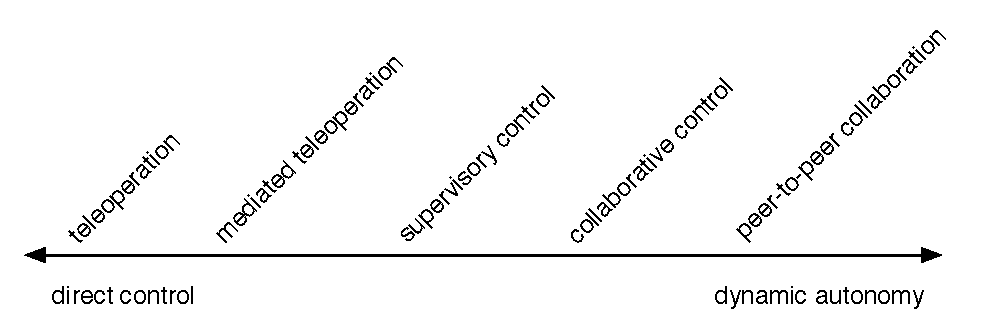
\includegraphics[width=5in]{images/autonomy.pdf}
\caption{Scale of Robot Autonomy\label{fig:autonomy}}
\end{center}
\end{figure}

% Awk. -ek
Robots, as they presently exist, have a fairly limited set of autonomous actions available. As a result, most interfaces, currently, are artificially conservative in their autonomy due to limitations in artificial intelligence. As research into artificial intelligence and machine learning grows, a much more diverse set of autonomous behaviors will inevitably become available. As user interface designers, we are tasked to create extensible interfaces to support future behaviors.

The Robot Interactive Display Environment, also known as RIDE, employs a dynamic approach known as sliding autonomy. This allows the human and the robot to change the level of autonomy as needed. RIDE allows the human to increase or decrease the level of autonomy on a per robot basis. In contrast, the robots are capable of only decreasing the level of autonomy. For illustration purposes, consider a robot that explores a warehouse. If the robot planned a poor navigation path, a user could manually specify the waypoints of an optimal path. If the robot is unable to complete the specified path due to an obstruction in the path, the robot could ask the user to directly teleoperate around the obstacle. Once free of the obstruction, the user would input a new set of goal coordinates and allow the autonomous navigation system to resume control.

% Needs tightening -ek
While the RIDE application does not specify any restrictions, I have elected to restrict the scope of my thesis to allow for a more careful examination of environmental searching within the range of supervised autonomy. In Section~\ref{section:futurework} I explain how these principles of RIDE could be adapted to support more autonomous behavior.

\subsection{Information Exchange}
\label{sub:info_exchange}
The nature of information exchange defines the flow of data between the human and the robot. What information is provided, how it is represented, and when it is communicated are all properties of the interface design. This encompasses low-level communication of navigation and sensor data as well as high-level commands sent from the human. 

The purpose of visualization interfaces is to represent the one-way exchange of information from the robot to humans. This data typically includes location information, laser or sonar readings, battery readings, accelerometer readings, and map data. Original interfaces were written to be accessible programatically. These interfaces were slowly adapted to display sensor data graphically, but the resulting interfaces were disjoint and required operator training. Examples of these 2D user interfaces can be seen in Figure~\ref{existing-robot-ui}.

In 2007 Dr. Curtis Nielsen introduced an ecological user interface with the goal of combining sensor data into a single, integrated display. Nielsen designed his interface to for effective teleoperation, the technique of controlling a robot remotely. In his study, Nielsen compared an integrated 3D user interface to a simple 2D user interface for several environment searching tasks. The 3D user interface displayed combined sensor data through a single viewport while the 2D user interface displayed the same data through individually. The study found the 3D interface decreased collisions and decreased task completion time. \cite{Nielsen_Teleoperation}

Nielsen attributes the success of the 3D interface to improved situational awareness. The observed effect of situational awareness and context on interface effectiveness is congruous with the findings of other researchers. \cite{Nielsen_Teleoperation}

A limitation of Nielsen's interface is that it's focus on teleoperation leaves the robot without autonomy. While teleoperation may be optimal for single robot environments it does not allow for concurrent robot control. This limitation requires an human operator for every active robot.

We adapted several elements from the Nielsen's ecological user interface in our design of RIDE. We designed the user interface to display inside a single viewport to avoid splitting the user's attention. We also procedurally construct a 3D world using the map and sensor data. This rich user experience allows the user visually perceive the state of the world as the robot perceives it. Finally, we introduced several new concepts to improve upon the weaknesses of the existing interfaces; a task system and a notification system.

We introduced an asynchronous task system allowing the human to directly command robots through a set of predetermined tasks. A robot may run only one single task at a time, and receiving a new task will replace the previous task. The task system was written generically to allow each robot to provide actions appropriate to its hardware and software. Additional details on the implementation of the task system can be found in Section~\ref{subs:ui-supervisor}.

To complement the task system, a notification system was also introduced. The notification system allows the robot to communicate with the human. The design of the notification system was enables the robot to select the importance of the message, and it permits the human to filter messages by importance. This gives the human operator the ability to ignore routine informational messages while still receiving urgent messages. An example notification is shown in Figure~\ref{fig:ride-notification}. The example shows the robot self-reporting that it has discovered a box, it's goal in this search and rescue scenario.

\begin{figure}[ht]
\begin{center}
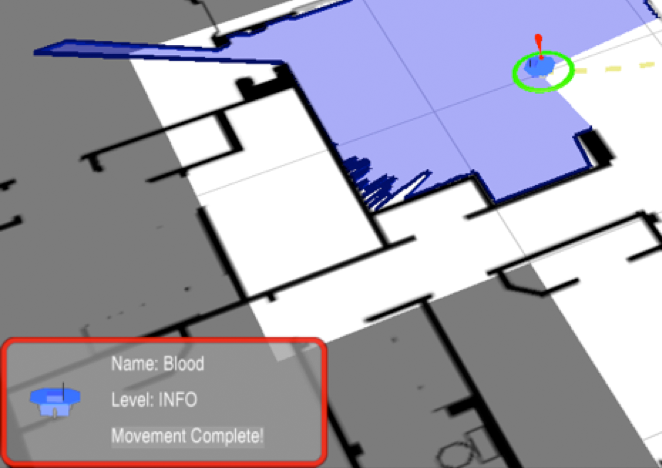
\includegraphics[width=6.10in]{images/ride-notification.png}
\caption{RIDE Notification Example\label{fig:ride-notification}}
\end{center}
\end{figure}

\section{RIDE User Interface}

The core of the RIDE user interface is the concept of sliding autonomy. In order to accomplish effective sliding autonomy, RIDE takes several cues from the video game industry. In our design phase, we decided to separate the user interface into two segments, the supervisor mode and the direct mode. The ``supervisor mode'' relies on robot to perform actions autonomously and report the information back to the human as appropriate. The ``direct mode'' allows the user to directly teleoperate a robot. By including both control styles, the user is given flexibility to use the most appropriate control mode for a given situation.

In addition to switching the control schemes between modes, we also change the fidelity of information exchanged. We found that providing streaming video for each robot was taxing not only on the network bandwidth but also on the human's perception. The movement from the video would draw the users eye to several places on the screen making effective management difficult. To combat this problem reduce the number of available sensors in the supervisor mode. When a user wishes to inspect a region with higher fidelity or the user wishes to teleoperate the robot, switching into the direct mode enables all sensors for the current robot. This design decision seemed to be fairly intuitive as will be explained in Section ??.

The basic RIDE user interface can be seen in.
\begin{figure}[ht]
\begin{center}
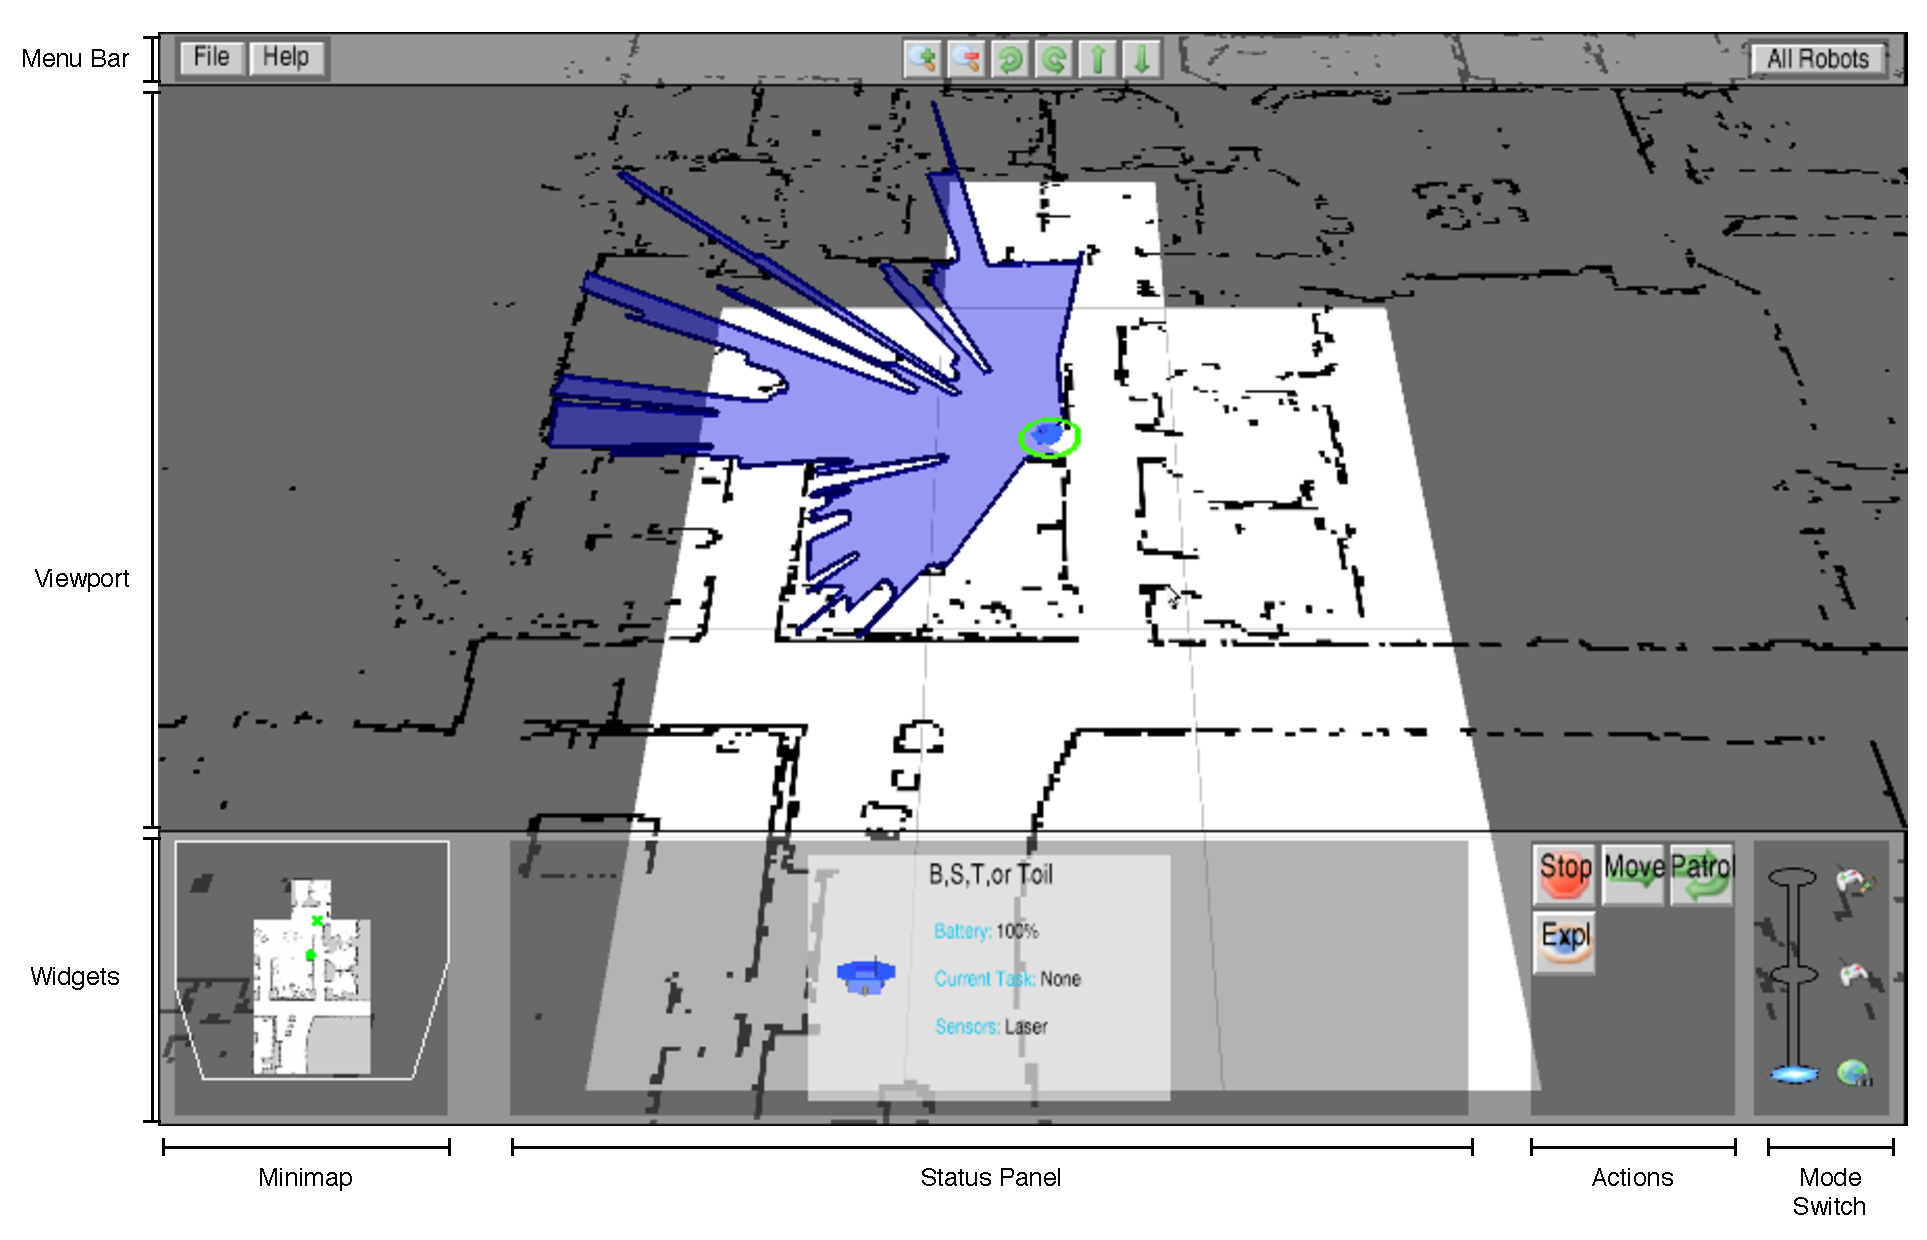
\includegraphics[width=6.10in]{images/ride-ui.pdf}
\caption{RIDE User Interface: Supervisory Mode\label{fig:ride-ui}}
\end{center}
\end{figure}
% In the next two subsections, I will discuss the design decisions for each user interface mode and the video game genre that inspired the interface. \textbf{I DON'T KNOW WHAT ELSE TO WRITE HERE, POSSIBLY CUSTOMIZATION?}.
% TODO: Introduce UI 


\begin{table}[ht]
\label{tab:ui-widgets}
\begin{center}
    \begin{tabular}{ | p{4cm} | l | l | l |}
    \hline
    \textbf{Mode} & \textbf{Left Widget} & \textbf{Center Widget} & \textbf{Right Widget} \\ \hline
    Direct Control & Mini-map & Information Panel & Proximity Panel \\ \hline
    Supervisory Control (Single Robot) & Mini-map & Status Panel & Action Panel \\ \hline
    Supervisory Control (Multiple Robots) & Mini-map & Group Panel & Action Panel \\ \hline
    \hline
    \end{tabular}
    \caption{RIDE User Interface Widgets}
\end{center}
\refstepcounter{table}
\end{table}

\subsection{Direct Control}

The direct control mode sets up a high fidelity of information exchange between the human and the robot as the user teleoperates the robot. Due to the large amount of prior work in the field of interfaces for teleoperation. We searched for video game design elements that would compliment the existing interfaces. While there are several styles of video game that we could draw on for inspiration, we decided to base our direct control mode off of ``open environment games.''

While not a genre in its own right open environment, or sandbox, games define a style of gameplay. Instead of the story following a predetermined linear path, the player is instead able to explore a world with the story unfolding around them. This style of gameplay is harolded by some as the future of games. Putting aside the narrative aspect of open environment games, the design elements that they employ have direct applicability to robotic interfaces.

The interfaces of open environment games are usually fairly minimal preferring leave most of the user interface available for camera display. The few user interface elements that do exist are typically semi-transparent to allow the user to see through UI components to the map. We applied this principal to all user interface components in RIDE by applying a small amount of alpha transparency. You can see an example of the transparency looking at the floor behind the user interface elements at the bottom of the screen in Figure~\ref{fig:ride-ui}.

In most open environment games, a third person camera follows behind the player's avatar. While controls exist that allow the user to manually rotate the camera, most gameplay occurs with default camera positioning. This camera control style is the inspiration behind our third-person direct control mode. The user uses the arrow keys on the keyboard to move the robot in a given direction and uses the mouse to rotate the camera as needed.

A common component of most open environment games is a minimap which allows users to orient themselves with relation to the ``world''. In video games, important characters, landmarks, and other notable locations may be displayed in the minimap. We added a minimap to the lower right hand corner of the RIDE user interface. The minimap is a component common to both the direct and supervisory control interfaces and we feel strongly that the minimap's location on screen should remain in the same location for both modes.

\subsection{Supervisory Control}
\label{subs:ui-supervisor}

The supervisory control interface is what set's RIDE apart from the interfaces described in the prior work. Unable to find any large scale control interfaces within the realm of robots, instead we looked at the video game industry for inspiration.

Our search led us to the genre of Real-time strategy games (RTS). RTS games are full genre in the world of computer and video games. The goal of real-time strategy games is to effectively control your units to achieve a specified goal. Often these goals require the user to control units across a large  map. Real-time strategy games stress a users ability coordinate large numbers of units in a short amount of time. 

RTS games use an isomorphic top-down view to display a large section of the environment at a time. The map can be navigated using either the keyboard or the mouse. Placing the moue pointer on the edge of the screen will translate the camera in the given direction. The keyboard can also be used directly manipulate the camera through both translation and rotation. An example user interface for a simple real time strategy can be seen in Figure ??. 

The control scheme for RTS games is a ``point and click'' style. The player begins by selecting a unit by left clicking on a unit in the viewport. Internally the RTS game uses ray projection to determine which selectable object, if any, was selected. The user interface will update denote a selected unit by updating the on-screen user interface components and marking the unit in the viewport. If no unit could be found any currently selected objects will become deselected.

We found that real time strategy games included their own task system similar to the task system described in Section ??. Furthermore, realtime strategy games support the control of heterogenous unit types. In the video games,  each unit type has separate abilities, strengths, and weaknesses. We wanted a way to visualize this information in the user interface without cluttering the main viewport during normal use. We developed two user interface widgets to represent the abilities, strengths, and weaknesses of each robot visually. 

The first element known as the ``information panel'' can be seen in Figure ??. When a robot is selected, the information panel shows a listing of the robot's name, type, battery status, current task, and a list of sensors. A small 3D mockup of the front of the robot is also displayed to visually represent the make of the robot.

The second panel developed for the supervisory mode was the ``action panel.'' The action panel displays a list of buttons representing available actions for the selected robot. This list of actions is populated from what the robot self-reports actions it can perform. The implementation details of how actions are auto-discovered is briefly covered in Section ??. Clicking on a button will prompt for any additional arguments, such as asking the user to click on a position, and then send the task instruction to the robot. In our development we found that visualizing a confirmation helped improve clarity of what instructions were given to the robot. As an example when the user instructs a robot to move to a specific destination, the user interface will blink the target icon twice on the destination.  

In our study of RTS games, we found that players would organize units into heterogenous groups such that the individual units complimented each other's strengths and weaknesses. This required an interface that allows a user to select multiple robots at the same time and then command the group effectively.

When a user wishes to select a group of robots, instead of a single left click the user may left click and drag a rectangle around the robots he or she wishes to select. Much like single unit selection a detailed information panel will display relevant data about the robot. However, instead of showing detailed information on a single robot, the the ``information panel'' will be updated to show basic information on group as a whole. The information panel displays a 3D mockup for each robot currently selected and the name of the robot. The user may move the mouses on top of the 3D mockup to obtain additional information about the robot.

In addition to the information panel, the ``action panel'' also has a slight change in behavior. The action panel selects the union of set of actions available to each robot. RTS games provided a base set of actions that all controllable units must be able to perform, ``Stop'' and ``Move''. We require the same two actions to be available for all robots in RIDE. The advantage of requiring the move command for all robots is that we can use a shortcut found in most RTS games. When a robot is selected -- instead of click on the move button and then clicking on a destination, the user need only right click on the destination on the ground.

% Need more

% RTS view
% Higher concurrency / lower fidelity
% 
% \begin{figure}[ht]
% \begin{center}
% 
\includegraphics[width=3.5in]{images/placeholder.png}
% \caption{RIDE Supervisory Control\label{fig:ride-ui-super}}
% \end{center}
% \end{figure}
% 
% 
% % FPS view
% % Single concurrency / high fidelity
% 
% \begin{figure}[ht]
% \begin{center}
% 
\includegraphics[width=3.5in]{images/placeholder.png}
% \caption{RIDE Direct Control\label{fig:ride-ui-direct}}
% \end{center}
% \end{figure}

%!TEX root = karulf-thesis.tex
\chapter{Implementation}

%% Unused!
% RIDE allows the human to increase or decrease the level of autonomy on a per robot basis. In contrast, the robots are capable of only decreasing the level of autonomy.

% Needs tightening -ek
%While the RIDE application does not specify any restrictions, I have elected to restrict the scope of my thesis to allow for a more careful examination of environmental searching within the range of supervised autonomy. In Section~\ref{section:futurework} I explain how these principles of RIDE could be adapted to support more autonomous behavior.


\section{User Interface}

The core of the RIDE user interface is the concept of sliding autonomy. In order to accomplish effective sliding autonomy, RIDE takes several cues from the video game industry. In our design phase, we decided to separate the user interface into two segments, the supervisor mode and the direct mode. The ``supervisor mode'' relies on robot to perform actions autonomously and report the information back to the human as appropriate. The ``direct mode'' allows the user to directly teleoperate a robot. By including both control styles, the user is given flexibility to use the most appropriate control mode for a given situation.

In addition to switching the control schemes between modes, we also change the fidelity of information exchanged. We found that providing streaming video for each robot was taxing not only on the network bandwidth but also on the human's perception. The movement from the video would draw the users eye to several places on the screen making effective management difficult. To combat this problem reduce the number of available sensors in the supervisor mode. When a user wishes to inspect a region with higher fidelity, switching into the direct mode enables all sensors for the current robot. This design decision seemed to be fairly intuitive as will be explained in Section ??.

\begin{figure}[ht]
\begin{center}
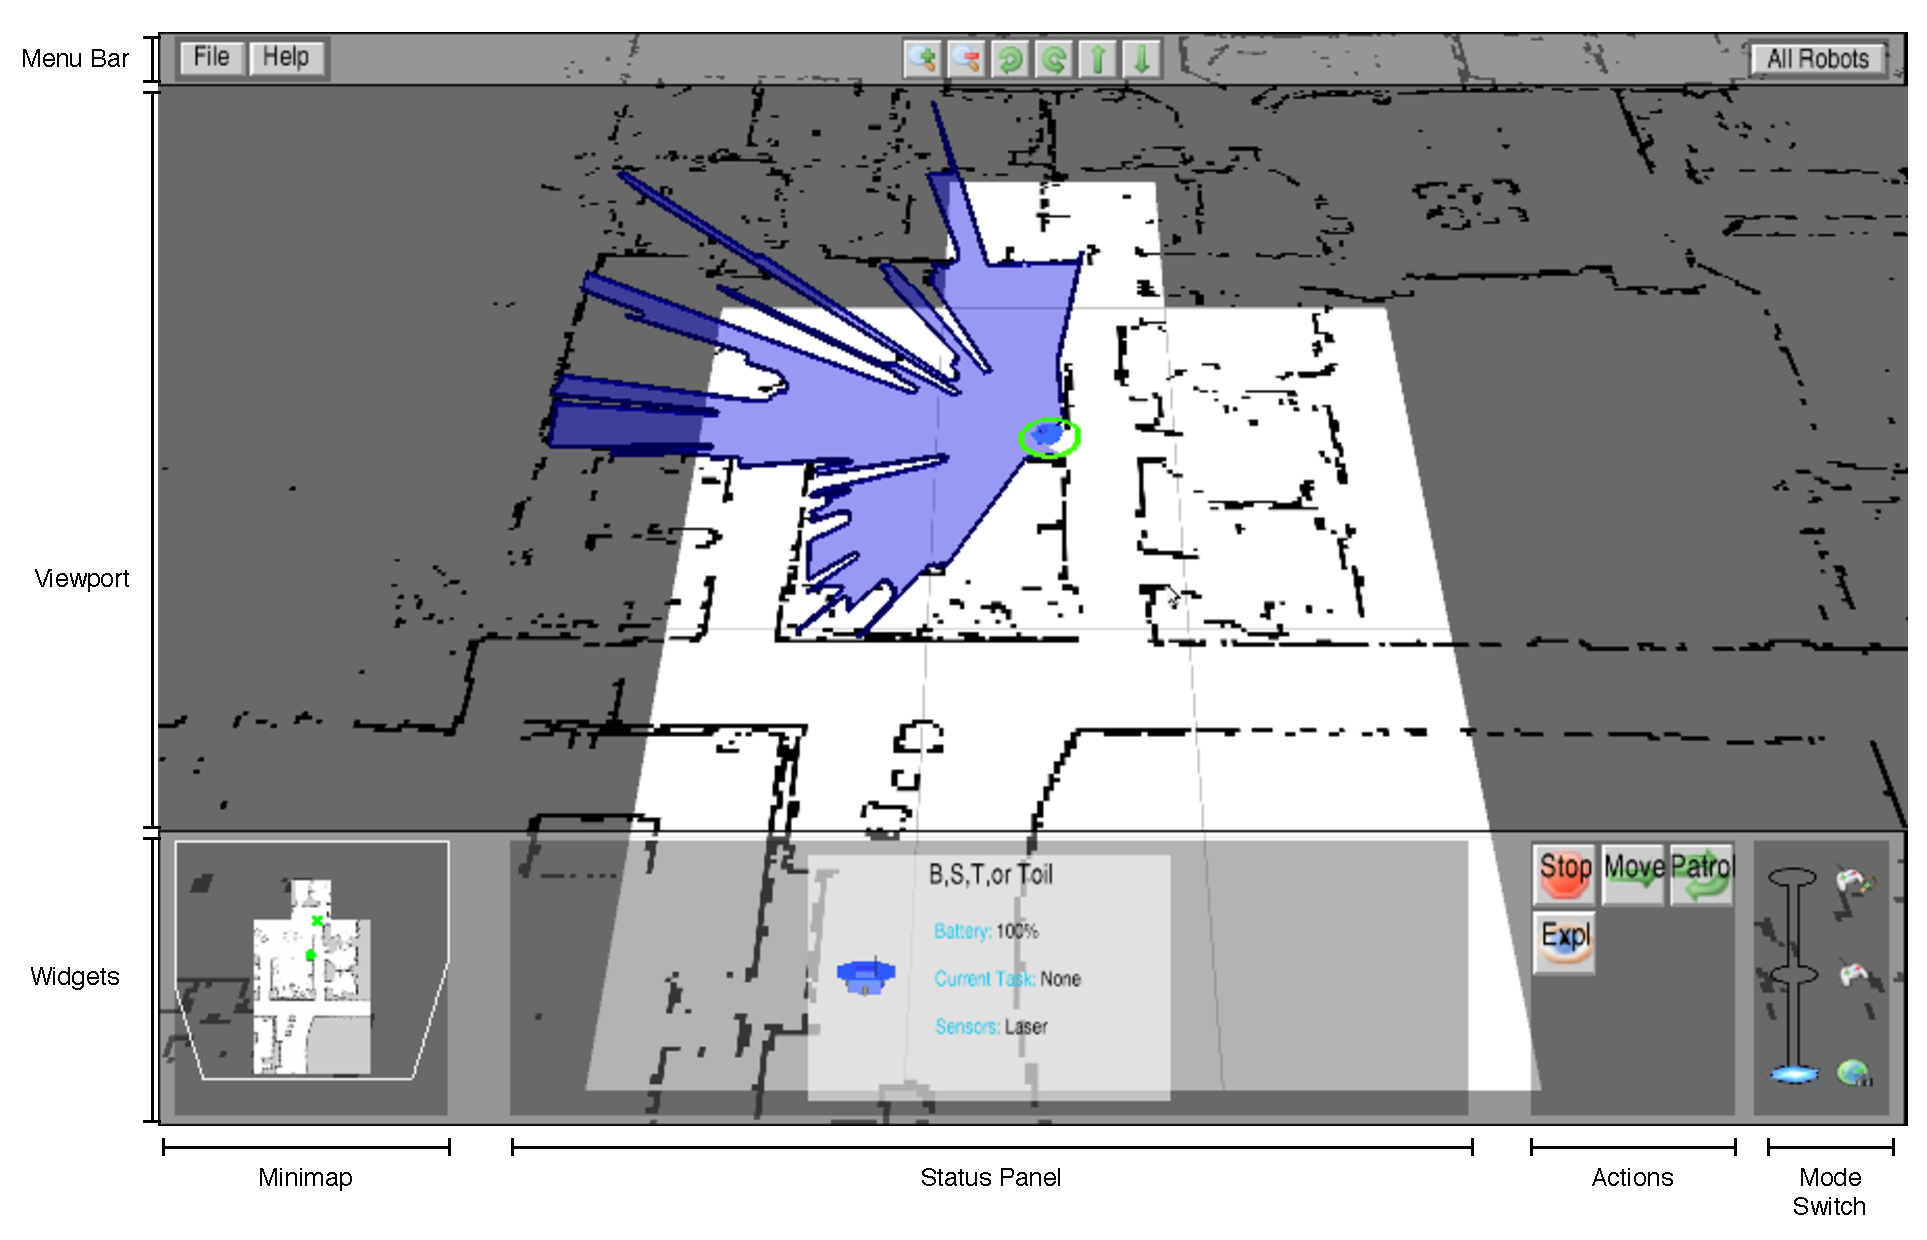
\includegraphics[width=6.10in]{images/ride-ui.pdf}
\caption{RIDE User Interface: Supervisory Mode\label{fig:ride-ui}}
\end{center}
\end{figure}

The screenshot figure in Figure~\ref{fig:ride-ui} shows the RIDE supervisory control mode with annotated descriptions of the user interface elements. The viewport is the main portion of the display. The viewport changes camera perspective based on the control mode, either locked behind the robot in the direct control mode or user operated in the supervisory interface. We took care to add alpha transparency to all user interface elements to prevent obstructing the viewport.

The menu bar at the top of the screen, remains static between the two control modes. The various menus allow for customization of the user-interface on a global and per-robot basis. These settings can be saved, and restored in future sessions. There are also menu bar buttons to control the camera viewpoint and zoom level, toggle the sensor information displayed, and to list all currently known robots.

At the bottom of the screen, the widget panel is displayed. The widget panel always contains a left, center, and right widget. A widget to change the display mode is always locked to the far right of the widget bar. Table~\ref{tab:ui-widgets} describes the widgets displayed based on the state of the interface.

\begin{table}[ht]
\label{tab:ui-widgets}
\begin{center}
    \begin{tabular}{ | p{4cm} | l | l | l |}
    \hline
    \textbf{Mode} & \textbf{Left Widget} & \textbf{Center Widget} & \textbf{Right Widget} \\ \hline
    Direct Control & Mini-map & Information Panel & Proximity Panel \\ \hline
    Supervisory Control (Single Robot) & Mini-map & Status Panel & Action Panel \\ \hline
    Supervisory Control (Multiple Robots) & Mini-map & Group Panel & Action Panel \\ \hline
    \hline
    \end{tabular}
    \caption{RIDE User Interface Widgets}
\end{center}
\refstepcounter{table}
\end{table}

\subsection{Supervisory Control}
\label{subs:ui-supervisor}

The supervisory control interface is what set's RIDE apart from the interfaces described in the prior work. Unable to find any large scale control interfaces within the realm of robots, instead we looked at the video game industry for inspiration. Our search led us to the genre of Real-Time Strategy games (RTS). 

As mentioned in Section~\ref{sub:RTS_games}, RTS games employ a top-down view of the world to control many units. We found that real time strategy games included their own task system. Furthermore, realtime strategy games support the control of heterogenous unit types; each unit type has separate abilities, strengths, and weaknesses. We wanted a way to visualize this information in the user interface without cluttering the main viewport during normal use. We developed two user interface widgets to represent the abilities, strengths, and weaknesses of each robot visually.

The first element known as the ``information panel'' can be seen in Figure ??. When a robot is selected, the information panel shows a listing of the robot's name, type, battery status, current task, and a list of sensors. A small 3D mockup of the front of the robot is also displayed to visually represent the make of the robot.

The second panel developed for the supervisory mode was the ``action panel.'' The action panel displays a list of buttons representing available actions for the selected robot. This list of actions is populated from what the robot self-reports actions it can perform. The implementation details of how actions are auto-discovered is briefly covered in Section ??. Clicking on a button will prompt for any additional arguments, such as asking the user to click on a position, and then send the task instruction to the robot. In our development we found that visualizing a confirmation helped improve clarity of what instructions were given to the robot. As an example when the user instructs a robot to move to a specific destination, the user interface will blink the target icon twice on the destination.  

In our study of RTS games, we found that players would organize units into heterogenous groups such that the individual units complimented each other's strengths and weaknesses. This required an interface that allows a user to select multiple robots at the same time and then command the group effectively.

When a user wishes to select a group of robots, instead of a single left click the user may left click and drag a rectangle around the robots he or she wishes to select. Much like single unit selection a detailed information panel will display relevant data about the robot. However, instead of showing detailed information on a single robot, the the ``information panel'' will be updated to show basic information on group as a whole. The information panel displays a 3D mockup for each robot currently selected and the name of the robot. The user may move the mouses on top of the 3D mockup to obtain additional information about the robot.

In addition to the information panel, the ``action panel'' also has a slight change in behavior. The action panel selects the union of set of actions available to each robot. RTS games provided a base set of actions that all controllable units must be able to perform, ``Stop'' and ``Move''. We require the same two actions to be available for all robots in RIDE. The advantage of requiring the move command for all robots is that we can use a shortcut found in most RTS games. When a robot is selected -- instead of click on the move button and then clicking on a destination, the user need only right click on the destination on the ground.

When porting the user interface from RTS games to human-robot interaction, we were able to re-use many of the existing design elements: unit selection, grouping, the action system, and mini-map. We also found that we needed to display additional elements: sensor visualization, coverage maps  decided to visualize additional sensor information when displaying robotic units. 


% Need more

% RTS view
% Higher concurrency / lower fidelity
% 
% \begin{figure}[ht]
% \begin{center}
% 
\includegraphics[width=3.5in]{images/placeholder.png}
% \caption{RIDE Supervisory Control\label{fig:ride-ui-super}}
% \end{center}
% \end{figure}
% 
% 
% % FPS view
% % Single concurrency / high fidelity
% 
% \begin{figure}[ht]
% \begin{center}
% 
\includegraphics[width=3.5in]{images/placeholder.png}
% \caption{RIDE Direct Control\label{fig:ride-ui-direct}}
% \end{center}
% \end{figure}

\subsection{Direct Control}

The direct control mode sets up a high fidelity of information exchange between the human and the robot as the user teleoperates the robot. Due to the large amount of prior work in the field of interfaces for teleoperation. We searched for video game design elements that would compliment the existing interfaces. While there are several styles of video game that we could draw on for inspiration, we decided to base our direct control mode off of ``open environment games.''

While not a genre in its own right open environment, or sandbox, games define a style of gameplay. Instead of the story following a predetermined linear path, the player is instead able to explore a world with the story unfolding around them. This style of gameplay is harolded by some as the future of games. Putting aside the narrative aspect of open environment games, the design elements that they employ have direct applicability to robotic interfaces.

The interfaces of open environment games are usually fairly minimal preferring leave most of the user interface available for camera display. The few user interface elements that do exist are typically semi-transparent to allow the user to see through UI components to the map. We applied this principal to all user interface components in RIDE by applying a small amount of alpha transparency. You can see an example of the transparency looking at the floor behind the user interface elements at the bottom of the screen in Figure~\ref{fig:ride-ui}.

In most open environment games, a third person camera follows behind the player's avatar. While controls exist that allow the user to manually rotate the camera, most gameplay occurs with default camera positioning. This camera control style is the inspiration behind our third-person direct control mode. The user uses the arrow keys on the keyboard to move the robot in a given direction and uses the mouse to rotate the camera as needed.

A common component of most open environment games is a minimap which allows users to orient themselves with relation to the ``world''. In video games, important characters, landmarks, and other notable locations may be displayed in the minimap. We added a minimap to the lower right hand corner of the RIDE user interface. The minimap is a component common to both the direct and supervisory control interfaces and we feel strongly that the minimap's location on screen should remain in the same location for both modes.

\subsection{Tasks and Notifications}
We adapted several elements from the Nielsen's ecological user interface in our design of RIDE. We designed the user interface to display inside a single viewport to avoid splitting the user's attention. We also procedurally construct a 3D world using the map and sensor data. This rich user experience allows the user visually perceive the state of the world as the robot perceives it. Finally, we introduced several new concepts to improve upon the weaknesses of the existing interfaces; a task system and a notification system.

We introduced an asynchronous task system allowing the human to directly command robots through a set of predetermined tasks. A robot may run only one single task at a time, and receiving a new task will replace the previous task. The task system was written generically to allow each robot to provide actions appropriate to its hardware and software. Additional details on the implementation of the task system can be found in Section~\ref{subs:ui-supervisor}.

To complement the task system, a notification system was also introduced. The notification system allows the robot to communicate with the human. The design of the notification system was enables the robot to select the importance of the message, and it permits the human to filter messages by importance. This gives the human operator the ability to ignore routine informational messages while still receiving urgent messages. An example notification is shown in Figure~\ref{fig:ride-notification}. The example shows the robot self-reporting that it has discovered a box, it's goal in this search and rescue scenario.

\begin{figure}[ht]
\begin{center}
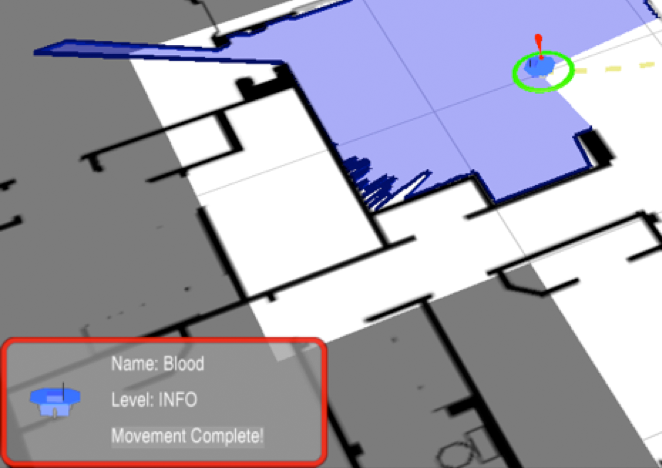
\includegraphics[width=6.10in]{images/ride-notification.png}
\caption{RIDE Notification Example\label{fig:ride-notification}}
\end{center}
\end{figure}


\section{Robot Operating System}
The Robot Operating System (ROS), developed by Stanford University and Willow Garage, is a specialized adaptation of the Common Object Request Broker Architecture (CORBA) design pattern for robotics software. This design decision gives ROS a modern distributed architecture that encourages small, reusable code.

The ROS architecture can be thought of as a directed graph. Software components are called ``nodes'' and are run in separate processes. This allows each node to be written using the most appropriate language to the task. As an example, a performance sensitive node could be written in C while a less demanding node could be written in Python for improved readability. At the time of writing ROS supports C++, Python, Java and Lisp.

% Nodes => Package
% Pacakages => Stack
% Stack => Repositories

\subsection{Topics and Services}
ROS provides a framework for connecting nodes together. Nodes can be connected together through a ``topic'' or through a ``service''. A topic is a named stream that supports multiple readers and writers. Nodes that write to a topic are known as ``publishers''. A publisher announces that it is publishing to one or more topics to the ``roscore'' node. 

The ``roscore'' node is a special node that is run when the ROS environment is initialized. It acts as a directory server maintaining a list of active nodes, topic, services, and configuration values.

Nodes that wish to read from a topic are known as ``subscribers''. Similar to publishers, a subscriber will announce it is listening to one ore more topics to the roscore node.

The roscore node continually informs subscribers of the location of publishers. This allows nodes to communicate directly without needing to contact the roscore node. Currently only TCP and UDP unicast sockets are supported, however future releases of ROS will include shared memory and multicast networking. A simple example of a ROS digraph can be seen in Figure~\ref{fig:middleware-ros}.

\begin{figure}[ht]
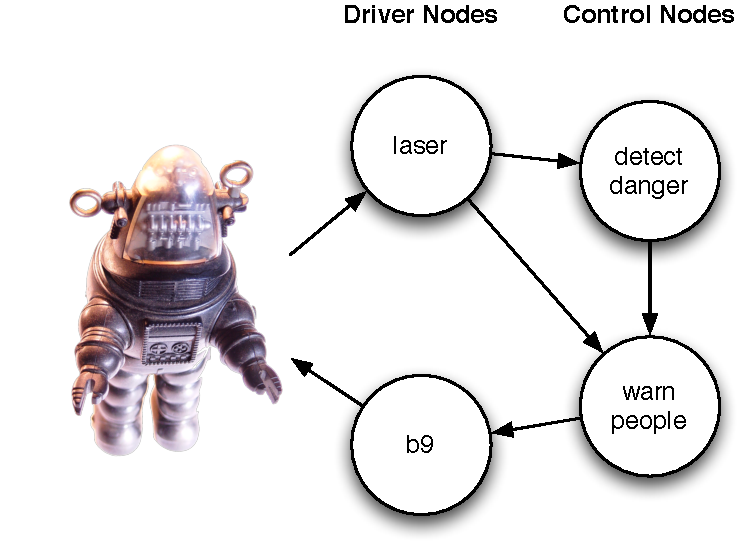
\includegraphics{images/middleware-ros.pdf}
\caption{Example ROS application\label{fig:middleware-ros}}
\end{figure}

The development of nodes can build on each other. Low-level hardware interface nodes communicate raw sensor and actuator messages. Unlike traditional robotic driver software, ROS allows the developer to break the control code up into several pieces. This modular interface allows code re-use of control code as well as driver code.

% TODO: correct acronym IDL
ROS also defines a common message format for communicating. Messages are defined using a independent-domain language (IDL) which in turn auto-generate serialization and deserialization code for supported languages. An example message file can be seen in Figure~\ref{fig:point}.

\begin{figure}[ht]
\makebox[\textwidth]{\hrulefill}
\begin{verbatim}
	# This contains the position of a point in free space
	float64 x
	float64 y
	float64 z
\end{verbatim}
\makebox[\textwidth]{\hrulefill}
\caption{Point.msg : Message representation of a 3D Point\label{fig:point}}
\end{figure}

\subsection{Kinematic Tree}
A large part of the complexity of robotic systems is transforming coordinate frame in a timely manner. ROS offers a special topic located at \verb!tf! and provides a cross-language library, also called ``tf'', to ease coordinate transformation tasks.

ROS builds a kinematic tree using data published to the \verb!tf! topic. Coordinate frames contain a timestamp, an object's name, the parent coordinate frame and the quaternion offset between the two. The tf package allows a developer to request a quaternion offset between two coordinate frames. 

In order to maintain a correct representation, the library automatically discards stale coordinate frame data. This requires objects to publish their location at a specified frequency. When all nodes are publish at an acceptable rate the full kinematic tree is accessible. A sample kinematic tree for a robot with a stero-vision rig mounted on-top of a pan-tilt unit can be seen in Figure~\ref{fig:tf-example}.

\begin{figure}[ht]
\begin{center}
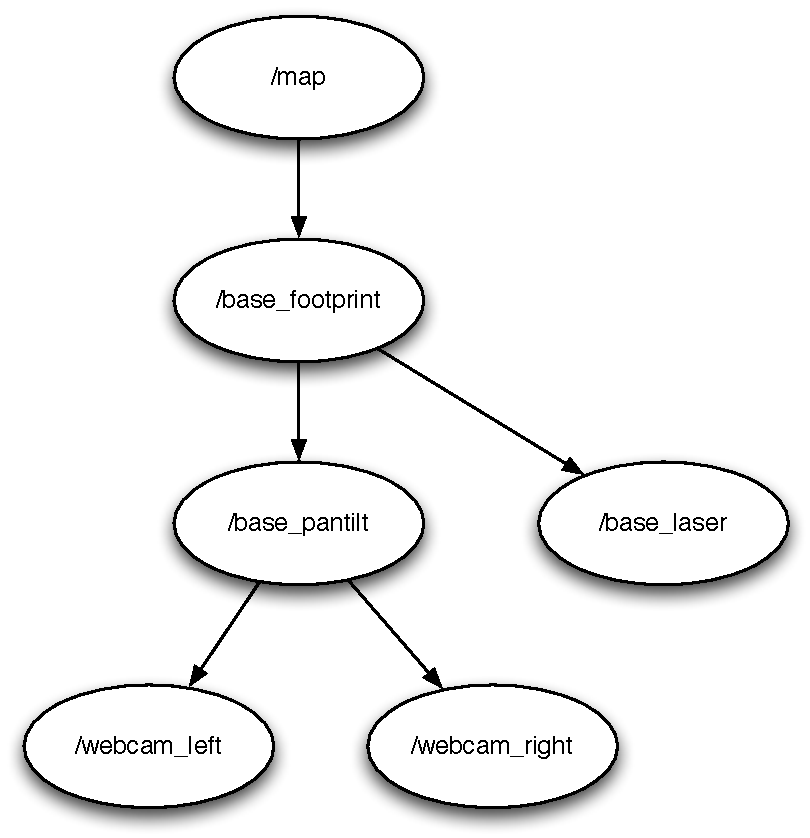
\includegraphics[width=3.5in]{images/tf-example.pdf}
\caption{Sample Kinematic Tree\label{fig:tf-example}}
\end{center}
\end{figure}

\section{RIDE Architecture}

ROS was originally designed for a single robot system. A node may only be attached to a single ROS graph (or ``realm''). RIDE is designed to work with large numbers of robots. Early on in the development cycle, I decided to stick to the model that realms are local to a robot. This allows robots to operate independently of connectivity to eachother, and does not require any changes to existing single-robot code bases. This design conflict required the development of a new node library called ``rosmultimaster''.

rosmultimaster allows a single node to connect to multiple realms using the native ROS python (rospy) codebase. rosmultimaster is multi-threaded library that provides both a synchronous and asynchronous interface. Further implementation details for rosmultimaster can be found in Appendix X % TODO: Appendix number

Using the rosmultimaster code-base, we developed RIDE to connect to each robot on startup, as well as a single mapping realm. A high level overview can be found in Figure X.X. The map realm acts as a central location to for map retrieval / updating. In the future, if ROS were to support peer-to-peer networking, a map could be dynamically built by stitching together several independent maps. 

% TODO: Generate high level figure

\subsection{Simulation Realm}
\label{sub:simulator}
I used a simulation environment, called ``rosstage'', to provide a consistent environment. The simulated system architecture is a superset of the regular RIDE architecture with the map realm acting as a full simulation realm and several additional topics being shared to the robot realms. An overview of the simulation architecture can be found in Figure~\ref{fig:ride-simulation-realm}.

\begin{sidewaysfigure}[ht]
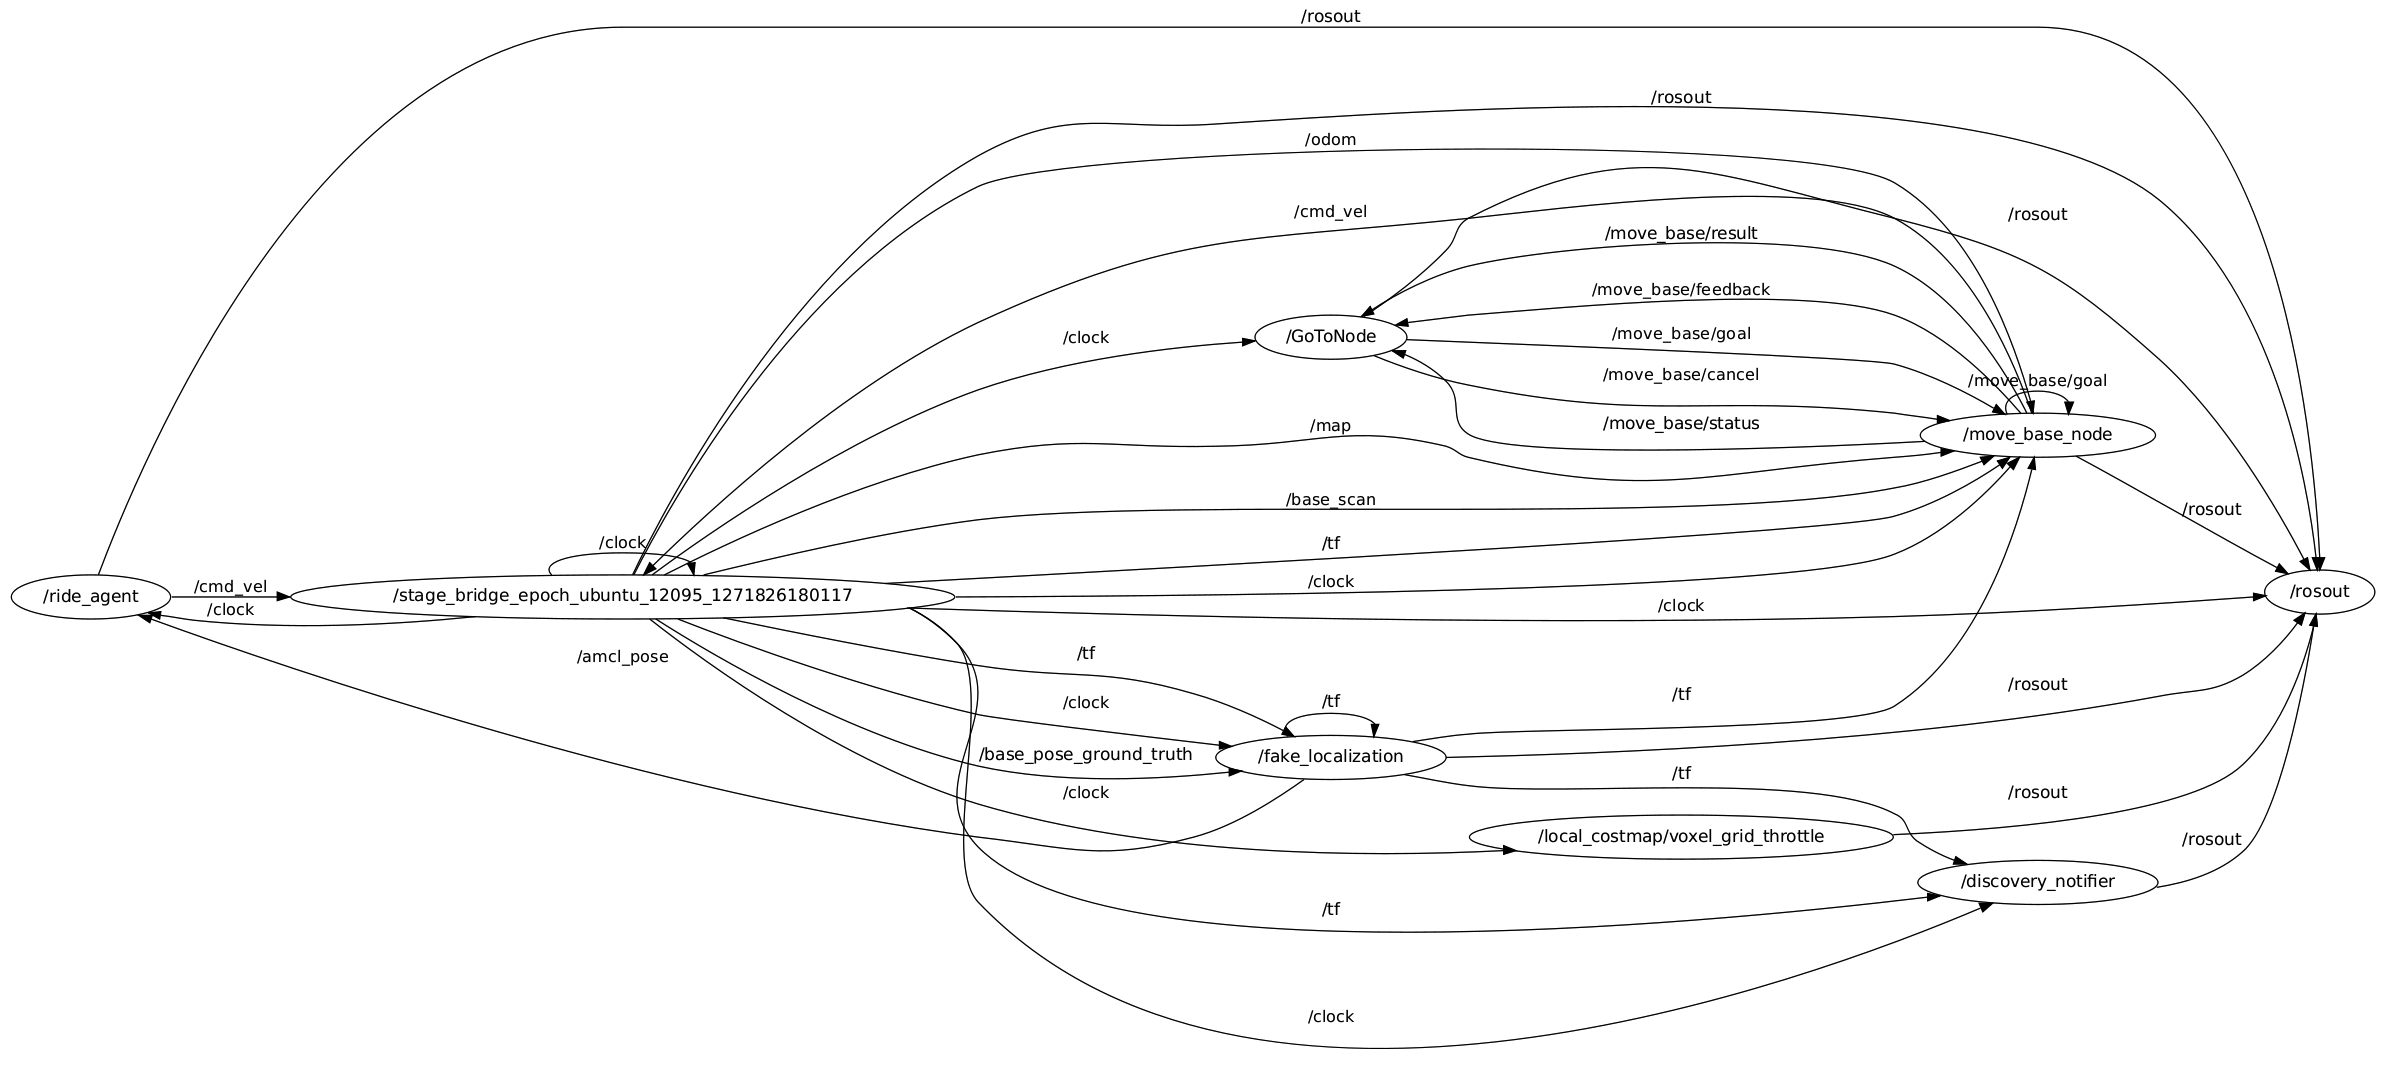
\includegraphics[width=\textwidth]{images/ride-simulation-realm.png}
\caption{Publish/Subscriber graph in RIDE Simulation Realm\label{fig:ride-simulation-realm}}
\end{sidewaysfigure}

\subsection{Robot Realm}
\label{section:robot-architecture}
RIDE uses a modular structure for controlling robots. Due to the topic system in ROS, this functionality can be written to work regardless of if the robot is simulated or physical. Each robot must provide position data for basic RIDE functionality. Beyond position data, the user can choose what sensors, actuators, and ``actions'' to provide.

Figure~\ref{fig:ride-robot-realm} demonstrates a simulated robot realm and the components to the most basic functionality. The robot must be able to orient itself with respect to the \verb!/map! coordinate frame. This typically requires a localization node like the Adaptive Monte-Carlo Localization (amcl) node when running on a physical robot or a fake localization node when running in simulation.

In addition to providing position data, the robot must expose a path planning node. ROS provides a navigation stack complete with a path planning node, called move\_base. Lastly, the robot must provide a way to directly control the movement of the robot allowing the user to ``drive'' a robot around freely.

% Discuss ride_agent
% Discuss GoToNode

\subsection{Panda3D Integration}

RIDE uses the popular 3D rendering engine Panda3D to display the virtual environment to the user. Panda3D is implemented in C++ for performance reasons, and provides a Python interface that we used to integrate with ROS. 

Like most rendering engines, Panda3D relies on a scene graph for rendering objects onto the screen. We kept a one-to-one mapping of objects in ROS's kinematic tree to objects in Panda3D's scene graph. This natural mapping proved to be simple and effective.

We developed a simple configuration file, using the YAML format, to let users configure which realms RIDE should connect to and what models to use when rendering objects from ROS's kinematic tree in the Panda3D scene graph. An example can be seen Figure~\ref{fig:tf-example}, where a single robot contains a laser range finder. Future work would remove the configuration file, moving the connection information into the user interface, and updating the RIDE protocol to provide dimensions and model information as needed.

% TODO: Insert figure: RRS / scene graph

Panda3D provides its own run loop for running tasks, processing events and updating the scene graph. For performance reasons, Panda3D does not use the native Python threading implementation so I chose to use the synchronous API offered by rosmultimaster. I then added one background task per rosmultimaster instance to Panda3D's task manager. The rosmultimaster tasks were called at a specified frequency designed to keep latency low and framerate high.

\chapter{User Study}

\section{Testing Procedures}

\section{Results}
In our post-experiment questionnaire, sever users remarked that the keyboard and mouse bindings in the supervisor interface were counter-intuitive. They felt that moving the camera should be done with the keys or the keyboard, and rotating the camera should be a function of a mouse click and drag event.
\chapter{Conclusion}

\section{Future Work}
\label{section:futurework}
%!TEX root = karulf-thesis.tex
\chapter{Conclusion}

We propose applying techniques and design elements from video games to address weaknesses in existing human-robot interfaces. We submitted RIDE, an interface for controlling heterogenous robot teams using design elements from video games. We introduced the concept of ``sliding autonomy'' to allow the human operator and the robot to vary the degree of robot autonomy dependent on the situation. We presented an overview of the implemented system, RIDE, using the ROS middleware framework. Finally we present the results of some preliminary user studies. Though the results of the user studies were mixed, we remain confident that refinements to the interface design and the user study process will provide clear results in future work.

\section{Future Work}
\label{section:futurework}
Observing the user interface use during the user studies revealed several weak points in our implementation. We believe that small enhancements to RIDE will greatly benefit the end user experience. % The modifications are broken into two categories: user interface changes and middleware changes.
We identified three major changes to our user interface: enhancing the ecological interfaces and creating actionable notifications.

In Section~\ref{sub:info_exchange} we introduced Nielsen's prior work designing ecological interfaces for robotics. While the paper was a large influence on our design work, we feel our interface would benefit from additional visual cues. In their proposed UI, Nielsen extruded the known elements from the coverage map vertically to create an approximate three dimensional representation. \ref{Nielsen_Teleoperation} In our original design, we rejected this design element as we believed it misrepresented the third dimension to the user. However during user studies, users often mentioned it was difficult to position the camera for teleoperation while keeping the map visible.

During our user studies we also found that many users, especially users without prior robotics experience, found the robots to behave in a counter intuitive manner. As an example, the path planning algorithm we used in our study is weighted in a way that often chooses a longer, more circuitous route to avoid obstacles than a more direct route that passes near obstacles. We believe that exposing more behavioral information will reduce the cognitive load on users. Future versions of the RIDE application would benefit from adapting the prior work in visualizing autonomous navigation systems to the field of robotics.

% TODO: Sensor coverage map?

% TODO: Notifications

\section{Future User Studies}
\label{sec:futurestudy}
As noted in Section~\ref{sec:study-results}, the design of the preliminary user study introduced several mitigating factors that prevented a clear acceptance of our hypothesis. Though the study returned some results, we feel our hypothesis can be clearly demonstrated with a revised experimental design. We have identified the several major problems with our experimental design. We propose several modifications to address the problems with our preliminary research.

In our preliminary user study, our intent was to provide a common set of knowledge in terms of robotics and video game experience. Unfortunately, by providing this training we made the analysis between experience groups much more difficult. As a result, we have widened our target audience to include users without robotics experience. In future studies, we plan to limit our training to only include speak-aloud practice to avoid introducing any potential biases.

In addition to the problems in our pre-experiment preparation, we have identified several ways to improve upon the experimental design itself. The purpose of our experiments was to prove applying video game principles to HRI interfaces will improve usability. In order to prove our hypothesis, we used notification display as an independent variable and recorded completion time as a measure of usability. While this is a valid approach, we would like to refocus our experiment to directly test our ``blended autonomy'' interface by measuring cognitive load. 

In order to evaluate the blended autonomy approach, we will run a randomized three-condition within subject experiment. Instead of using notifications we will use the control modes as our independent variable. This gives us three conditions to test: only direct control, only supervisory control, and blended control. This would allow us to directly compare the given modes and record metrics on the blended control interfaces such as time spent in each mode and the number of mode switches.

As mentioned above while we can correlate successful task completion with improved usability, we would like to utilize a more direct metric. Researchers at the United States National Aeronautics and Space Administration (NASA) developed a metric for describing a human's workload while accomplishing a task. The metric, known as the ``Task Load Index'', is computed from a user's perceived workload on six sub-scales: mental demand, physical demand, temporal demand, performance, effort, and frustration. \cite{NASA_TLX} Our revised user study would ask participants to rate their workload on each of the Task Load Index's six sub-scales after each experiment. At the conclusion of the user study, we would ask users to answer the fifteen questions to determine the weighting of the sub-scales when computing the task load index. \cite{NASA_TLX20}

Given the context of testing the control modes using the NASA Task Load Index, we decided to modify the tasks to more accurately represent our use cases. The preliminary user study asked participants to find several boxes hidden randomly throughout a small house using two robots. We would like to add specificity to the roles participants will be pretending. We tell participants that several hikers are lost in the woods, the participant works for the Sheriff's office and they are controlling robots to assist in the search. A weakness in the preliminary study is that the robots were able to complete their task immediately, while most actions taken by a robot will require a non-zero amount of time to complete. In our scenario, we will ask participants to remain with the hiker and broadcast a notification beacon until a rescue crew arrives. We believe that by assigning a more difficult task, the differences between the user interfaces will become more pronounced.

\appendix                        % now we start appendicies
\chapter{The English Language and Other Confusing Things}
\label{app:english-language}

While this guide answers most questions about how to format a thesis, it does
not address questions about English grammar, use of abbreviations, punctuation,
spelling, and other confusing subjects.  Students should obtain a dictionary
and a style of grammar book to refer to as questions arise.  The dictionary is
important because most electronic spelling checkers are not complete and do not
contain definitions.  (You may also need to refer to some of the references you
cite for the spelling of technical terms.)  The grammar or style book is useful
for checking grammar and punctuation rules.  A good style manual contains
information about correct English usage as well as advice for preparing a
manuscript.  \textit{A Manual for Writers of Term Paper, Theses, and
Dissertations}~\cite{Turabian} is one such concise and inexpensive manual based
on the lengthy and more expensive \textit{Chicago Manual of
Style}~\cite{ChicagoManual}.  

The following rules will help you avoid three mistakes frequently made
by students:
\begin{itemize} 
 \item Hyphenated words must begin and end on the same page.

 \item When a page break falls in the middle of a paragraph, at least
two lines of text from that paragraph must appear on the second page.

 \item At least one line of text from a section or subsection must
appear on the same page as the title of that section or subsection.
\end{itemize}

%%% Local Variables: 
%%% mode: latex
%%% TeX-master: "thesis-main"
%%% End: 

\chapter{Procedures and Deadlines}
\label{app:procedures}

\paragraph{Deadlines}

At least one semester prior to the semester in which you believe you will
complete all requirements for your degree, please be sure to consult with your
department’s graduate administrative assistant or coordinator to be sure you
are aware of all requirements and deadlines with regards to the submission of
your thesis or dissertation.  Deadlines are printed in the course listings
schedule book and are posted online.  If you cannot make certain deadlines, you
may have to postpone your graduation accordingly.  In particular, a student
must file an ``intent to graduate'' form (via WebSTAC) by the published
deadline prior to any anticipated graduation date; otherwise, no degree can be
earned.  M.S.\ and D.Sc.\ students also have a special deadline by which they
must submit an initial hard copy draft of their thesis to Engineering Student
Services in Lopata 303 so that it can be reviewed for formatting.  After a
draft has been submitted for format review, an email will be sent to you within
48 hours detailing any changes that need to be made in the formatting of your
thesis or dissertation.  For M.S.\ and D.Sc.\ students, approval of your thesis
or dissertation formatting must be received prior to turning in the final
electronic and hard copy versions as described below.  

Ph.D.\ students must follow the requirements of the Office of Graduate Students
in Arts and Sciences (GSAS).  The GSAS office does not have special formatting
deadlines, but you should still contact that office if you have questions about
your formatting.

\paragraph{Oral Examination}

Each member of the oral examining committee must be given a copy of the thesis
or dissertation, in final form, in sufficient time to study it before the oral
examination.  Members of the examining committee have the right to request
rescheduling of the examination if these copies are not made available to them
at least one week in advance of the scheduled examination date.  Copier paper
may be used for these preliminary copies.

\paragraph{Electronic Submission}

After the oral defense, an M.S.\ or D.Sc.\ student is required to submit an
electronic version of his/her final thesis or dissertation in PDF format.  The
links can be found on the School of Engineering website under Information for
Graduate Students.   Click on the link for Thesis Submissions to submit a
Master's Thesis or click on the link for Dissertation Submissions to submit a
Doctoral Dissertation. The website for doctoral students submitting
dissertations requires students to choose among publishing and copyrighting
services offered, but the University permits students to make whichever choices
they prefer. Doctoral students are asked to submit a Survey of Earned
Doctorates separately to Engineering Student Services. 

Please note that the electronic submission of your thesis or dissertation
should be made by the stated deadline date on the current academic calendar and
prior to handing in the final hard copies as described below.  An administrator
in Engineering Student Services will review the electronic copy of your thesis
or dissertation and officially approve the submission online.  This electronic
version will be used for library publication and catalog purposes. In addition,
students typically must submit hard copies of the thesis or dissertation for
binding purposes (see below).  

\paragraph{Final Hard Copies}

After the oral defense and electronic submission, final copies of the thesis or
dissertation approved by the examination committee and department are to be
submitted to Engineering Student Services in Lopata 303 on or before the date
stated in the current academic calendar.

\begin{enumerate}
	\item	
	\textbf{Three} final copies (unless your department instructs you
	otherwise) must be printed using only one side on 8.5 $\times$ 11 inch
	white paper and minimum 20-pound weight. (Most printer and copier paper
	qualify, but a high-quality watermarked or 10--25\% cotton paper is
	recommended.) Print should be letter quality.  Copies submitted should
	\uline{not} be bound, stapled, clipped or hole-punched.  To avoid
	delays in publication, please make certain that the copies you submit
	include all pages of your thesis or dissertation.
	
	Each copy should be placed in a separate unsealed manila envelope with
	a copy of the \textbf{short title page} (see description below)
	securely taped to the outside of each envelope.

	\begin{list}{}{}
		\item \textit{%
		Engineering Student Services sends all three copies of your
		thesis or dissertation to West Campus Library.  The Library
		will have these copies professionally bound and sent back to
		your home department.  The home department will keep one copy
		and distribute one to your advisor.  The third copy will be
		mailed to you at your home address.  In order for you to
		receive your bound thesis or dissertation promptly, your home
		department must have your current mailing address.  On your
		``intent to graduate'' form you should input your ``address
		after graduation.''   Processing theses and dissertations takes
		time, so you may have to wait 3--6 months after your graduation
		date to receive your copy. 
		}
	\end{list}

	\item		
	\uline{\textbf{Short Title} page is a loose sheet containing} (1) a
	\uline{short title} of 35 letters or less (including spaces), (2) the
	author’s last name, (3) the degree, and (4) the year of its award,
	centered on the page and punctuated as in the example.\footnote{See the
	sample short title page for this document}    This short title sheet is
	to be taped securely to the outside of each manila envelope as
	described above.  This information lets the bindery know what to put on
	the spine of the bound copies.  The title will be truncated if longer
	than 35 characters.
	
	\item
	\textbf{Doctoral (D.Sc.) degree candidates} must complete the Survey of
	Earned Doctorates form and submit it with the 3 copies of your final
	dissertation. You can download the Survey of Earned Doctorates form
	from the School of Engineering's website under Graduate Student
	Information and Forms.

	\textbf{NOTE FOR PH.D.\ STUDENTS}:  Deliver all three copies of your
	dissertation to the GSAS Office.  See GSAS dissertation guidelines on
	their web site.
\end{enumerate}

%%% Local Variables: 
%%% mode: latex
%%% TeX-master: "thesis-main"
%%% End: 

% \chapter{Thesis Format Checklist}

\newcommand{\smallblank}{\underline{\hspace{0.25in}}\,}
\newcommand{\largeblank}{\underline{\hspace{0.75in}}\,}

{\footnotesize \textbf{NOTE: If you have significantly varied formatting from that
which is shown in this document, please complete this form and submit it to
Engineering Student Servcies when you submit your thesis for format review.}}

Author's Name:  \underline{\hspace{4.0in}} \\
Title page font:  \smallblank 12 pt \indent \smallblank 14 pt \\
Table of contents chapter titled font: \smallblank plain \indent \smallblank bold \\
First level table of contents indentation (0 to 0.5 inch): \largeblank \\  
Second level table of contents indentation (0 to 1 inch): \largeblank \\
Body text font: \smallblank 10 point \quad \smallblank 11 point \quad \smallblank 12 point \\
Body text line spacing: \smallblank 1.5 \quad \smallblank 2 \indent \\
Body text justification: \smallblank left \quad \smallblank full \\
Paragraph indentation (0 to 0.5 inch):  \largeblank \\
Chapter title position (1.5 to 3 inches below top edge):  \largeblank \\
\begin{tabular}{@{}lll}
Chapter title style: \smallblank with word ``Chapter'' & \multicolumn{2}{l}{\smallblank without word ``Chapter''} \\
Chapter title:  \smallblank (10 to 36 point) & \smallblank plain & \smallblank bold \\
& \smallblank centered & \smallblank left justified \\
Section heading: \smallblank (10 to 24 point) & \smallblank plain & \smallblank bold \\
& \smallblank centered & \smallblank left justified \\
Subsection heading:  \smallblank (10 to 18 point) & \smallblank plain & \smallblank bold \\
& \smallblank centered & \smallblank left justified \\
Unnumbered heading: \smallblank (10 to 14 point) & \smallblank plain & \smallblank bold \\
& \smallblank centered & \smallblank left justified
\end{tabular} \\
Label tables as: \smallblank Table \quad \smallblank Figure \\
Reference list style (parenthetical, etc.): \underline{\hspace{3.0in}}

%%% Local Variables: 
%%% mode: plain-tex
%%% TeX-master: t
%%% End: 

% \wrappedappendix{Special Notes for \LaTeX{} Users, Including a \\
	\hbox to 1.0in{}Demonstration of Wrapping Appendix Titles}
{Special Notes for \LaTeX{} Users, Including a Demonstration of Wrapping Appendix Titles}
%\chapter{Special Notes for \LaTeX{} Users}
\label{app:latex-notes}

\newcommand{\cmd}[1]{\texttt{$\backslash$#1}}

It is strongly recommended that you use this file as a template for your
thesis, since it greatly simplifies conforming to the required formatting
standards.

There are several important points that students using the \LaTeX{} version of
this template should verify before submitting a thesis.

\section{Front Matter}

Much of the front matter (i.e., the Roman numbered pages) is automatically
generated.  Use \cmd{renewcommand} command to customize the fields of these
templates.  For example,
\texttt{\cmd{renewcommand}$\{$\cmd{thesisauthor}$\}\{$your name here$\}$} will
customize the author name.

\sloppy
Most authors will need to customize the \cmd{thesismonth}, \cmd{thesisyear},
\cmd{thesisauthor}, \cmd{thesisauthorlastname}, \cmd{thesisdefensedate},
\cmd{thesistitle}, \cmd{thesisshorttitle}, \cmd{thesisdepartment},
\cmd{thesisfield}, \cmd{thesissupervisor}, and \cmd{thesiscommittee}
fields.  Examples of these can be seen in the sample \texttt{thesis-main.tex}
file.

\fussy
You must also specify \texttt{phdthesis}, \texttt{dscthesis}, or
\texttt{mastersthesis} when selecting the \cmd{documentclass}.  An
example can also be seen in the sample \texttt{thesis-main.tex} file.

\section{Table of Contents and Bibliography}

The Table of Contents is automatically generated.  \texttt{latex} should be run
twice in succession after making any changes to the Table of Contents.

Due to the way \LaTeX{} formats the Table of Contents, long appendix titles
will not automatically wrap and indent properly.  If you need to use a long
appendix title, you must manually wrap and indent the appendix's
table-of-contents entry.  The \cmd{wrappedappendix} command is defined in this
template to assist with this; an example is seen at the top of the sample
\texttt{thesis-appendixD.tex}.  This requirement only applies to appendix
titles: other section titles will automatically wrap properly, including
entries in the List of Tables and List of Figures.

If changes need to be made to the Table of Contents' formatting, you can use
the \cmd{addtocontents} command to insert some formatting commands
directly into the Table of Contents page.  More significant changes can be made
by editing the \texttt{.toc} file that \LaTeX{} automatically generates.
However, editing this file by hand is not recommended unless absolutely
necessary, since it will automatically be re-generated the next time \LaTeX{}
is run.

Like the Table of Contents, the Bibliography is automatically generated.  After
editing the bibliography file, you should run \texttt{latex}; run
\texttt{bibtex}; and re-run \texttt{latex} twice in succession.

\section{Widows and Page Breaks}

\LaTeX{} may create widows if you have a paragraph followed by a list.  To get
rid of this widow, you must force \LaTeX{} to break the page somewhere else.
Either insert a \cmd{newpage} command before the paragraph, or insert a
\cmd{samepage} command between the paragraph and the list.

\LaTeX{} may also create widows in the Tables of Contents.  You can force
\LaTeX{} to break the page in a more convenient location by inserting
\cmd{addtocontents$\{$toc$\}\{$\cmd{newpage}$\}$} before the corresponding
\cmd{chapter}, \cmd{section}, \cmd{subsection}, or \cmd{subsubsection} command
in the text.

Excluding these two situations, \LaTeX{} should not create orphans or widows.
However, in some situations it may place page breaks at strange places --- such
as several inches above the bottom margin --- in order to avoid creating
orphans or widows.  You can fix this by altering the \cmd{clubpenalty} or
\cmd{widowpenalty}, or by manually adding \cmd{newpage}s where \LaTeX{} guesses
incorrectly.


% A good place for the bibliography.
%
\bibliographystyle{plain}
\begin{spacing}{1.0}
\bibliography{./thesis-references}
\end{spacing}
\nocite{*}
%
% The Vita should be the last thing
%
\begin{thesisauthorvita}
%
% This is just a sample of what to do in a vita
%
%
%
% Sample  Vita
% This is done in a list environment.
%
% Personal heading
\begin{center}
{\large\thesisauthor}
\end{center}
%
% Need to 'fold' long labels
%
\newcommand{\vitalabel}[1]%
  {\raisebox{0pt}[1ex][0pt]
    {\makebox[\labelwidth][l]%
      {\parbox[t]{\labelwidth}{\hspace{0pt}\textbf{#1}}}}}
%
% Here's the list definition
%
\begin{list}
  {}%                                        nodefault label
  { \renewcommand{\makelabel}{\vitalabel}%   setting labels
    \setlength{\labelwidth}{100pt}%          label width
    \setlength{\leftmargin}{120pt}%
    \setlength{\itemindent}{0pt}%            don't indent first line of items
    \setlength{\parsep}{\baselineskip}%               space between paragraphs
    \setlength{\itemsep}{5pt}%               additional space between items
    }
\item[Date of Birth] July 19, 1986
\item[Place of Birth] Dayton, Ohio
\item[Degrees] B.S.\ Computer Science, December 2009 \\
	M.S.\ Computer Science, May 2010
\item[Professional\linebreak Societies]
  Association for Computing Machinery
% \item[Publications]
%   Student, I.\ D.\ (2005).\ \LaTeX{} document class for Sever Institute,
%   \textit{The \LaTeX{} J.} \textbf{10}(4):~323--336.
%   
%   Student, I.\ D.\ (2005).\ More \LaTeX{} wisdom, \textit{Another \LaTeX{} J}.
%   \textbf{42}(7):~100--101.
\end{list}
\flushright
\thesismonth\ \thesisyear


\end{thesisauthorvita}

\begin{thesisshorttitlepage}
\iffalse
{\small 

\textbf{NOTE:}	This is a sample of a ``short title'' page.  Please change the
line above to use an appropriate ``short title'' for your thesis, insert your
last name, and include your degree and year in which the degree will be earned.
Separate elements using commas, as illustrated in the sample above.
\uline{Your ``short title'' cannot exceed 35 characters, counting spaces}.  It
does not matter if there is a page number at the bottom of the page.  

\textbf{IMPORTANT:} This page should be printed and taped securely to each of
the three manila envelopes used to submit your final hard copies.  Remove this
page before submitting your final copies (i.e., this page should not be
included in either your electronic submission or your hard copy submissions).
See Appendix~\ref{app:procedures} for further details if necessary.
}
\fi
\end{thesisshorttitlepage}

%%% Local Variables: 
%%% mode: latex
%%% TeX-master: "thesis-main"
%%% End: 


\end{document}
